% !Mode:: "TeX:UTF-8"
\documentclass{article}
\usepackage{CJK}
\usepackage{graphicx}
\usepackage{subfigure}
%\usepackage{subfig}

\begin{document}
\begin{CJK}{UTF8}{gbsn}
	

	
\section{exp}

两张图片并列在一行(发现label无法引用到,这里也有讨论https://tex.stackexchange.com/questions/175184/using-cref-on-a-minipage-label)
\begin{figure}[!tbp]
	\centering
	\begin{minipage}[b]{0.4\textwidth}
		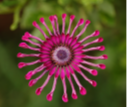
\includegraphics[width=\textwidth]{imgs/flower1.png}
		\label{fig:label1}
		\caption{Flower one.}
	\end{minipage}
	\hfill     % 这行如果去掉了,两张图片中间的空间就没有了
	\begin{minipage}[b]{0.4\textwidth}
		
\includegraphics[width=\textwidth]{imgs/flower2.png}
		\label{fig:label2}
		\caption{Flower two.}
	\end{minipage}
\end{figure}
	


法二:子图模式,用subfig包
\iffalse    subfig和subfigure包有冲突,不能共用
\begin{figure}%
	\centering
	\subfloat[label 1]{{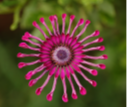
\includegraphics[width=5cm]{imgs/flower1.png} }}%
	\qquad
	\subfloat[label 2]{{
\includegraphics[width=5cm]{imgs/flower2.png} }}%
	\caption{2 Figures side by side}%
	\label{fig:example}%
\end{figure}
\fi


法三:用subfigure包
%\iffalse    subfig和subfigure包有冲突,不能共用
\begin{figure}
	\hfill
	\subfigure[Title A]{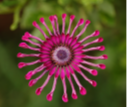
\includegraphics[width=5cm]{imgs/flower1.png}}
	\hfill
	\subfigure[Title B]{
\includegraphics[width=5cm]{imgs/flower2.png}}
	\hfill
	\caption{Title for both}
\end{figure}
%\fi



两张图并排,其中一张图还有两个子图
\begin{figure}[!tbp]
	\setlength{\abovecaptionskip}{0pt}
	\setlength{\belowcaptionskip}{0pt}
	\centering
	\begin{minipage}[b]{0.4\textwidth}
		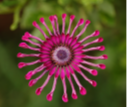
\includegraphics[width=\textwidth]{imgs/flower1.png}
		\caption{Flower one.}
	\end{minipage}
	\hfill
	\begin{minipage}[b]{0.55\textwidth}
		\subfigure[SL=0.5]{
			\label{fig:overall_cost_0.03} %% label for first subfigure
			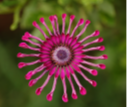
\includegraphics[width=0.31\textwidth]{imgs/flower1.png}
		}
		\subfigure[SL=0.5]{
			\label{fig:overall_cost_0.04} %% label for first subfigure
			
\includegraphics[width=0.31\textwidth]{imgs/flower2.png}
		}
		\caption{Flower two.}
	\end{minipage}
\end{figure}


\end{CJK}
\end{document}